\documentclass[tikz,border=2pt]{standalone}
\usepackage{amsmath}
\usetikzlibrary{arrows.meta}
\begin{document}
% Level curves f = 1, 4, 9 of f(x, y) = (x - 2)^2 + (y + 1)^2 (circles of radius 1, 2, 3 around
% (2, -1)); optim(c(0, 0), f2, method = "BFGS") starts at (0, 0), where f = 5, and returns (2, -1).
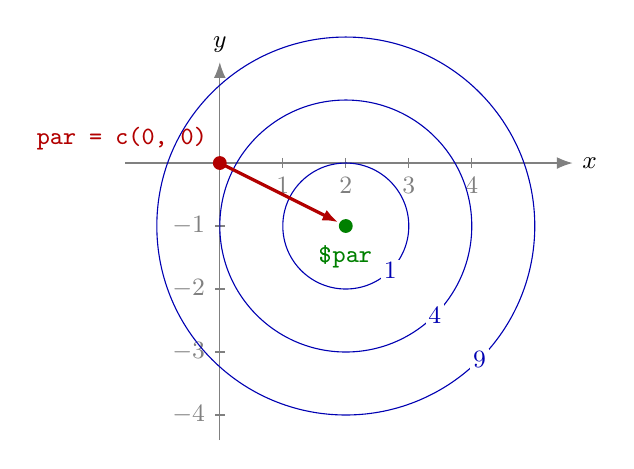
\begin{tikzpicture}[font=\small, >={Latex[length=2mm]}, x=0.8cm, y=0.8cm]
  \draw[->, gray] (-1.5,0) -- (5.6,0) node[right, black] {$x$};
  \draw[->, gray] (0,-4.4) -- (0,1.6) node[above, black] {$y$};
  \foreach \t in {1,2,3,4} \draw[gray] (\t,0.08) -- (\t,-0.08) node[below] {$\t$};
  \foreach \t in {-1,-2,-3,-4} \draw[gray] (0.08,\t) -- (-0.08,\t) node[left] {$\t$};
  \foreach \r/\v in {1/1,2/4,3/9} {
    \draw[blue!70!black] (2,-1) circle (\r);
    \node[blue!70!black, fill=white, inner sep=1pt] at ({2+\r*cos(-45)},{-1+\r*sin(-45)}) {$\v$};}
  \draw[->, very thick, red!70!black] (0,0) -- (1.88,-0.94);
  \fill[red!70!black] (0,0) circle (2.5pt);
  \node[red!70!black, anchor=south east] at (-0.05,0.05) {\texttt{par = c(0, 0)}};
  \fill[green!50!black] (2,-1) circle (2.5pt);
  \node[green!50!black, anchor=north] at (2,-1.15) {\texttt{\$par}};
\end{tikzpicture}
\end{document}
